% !TEX root = ./main.tex
\documentclass[a4paper]{article}
% Course language: use [english] or [german].
\usepackage[german]{ajnotes}
\title{\textbf{Betriebwirtschaftslehre — Marketing B}}
\begin{document}
    \maketitle
    % Attach the given problem sheet: drop it in this folder as sheet.pdf and
    % un-comment the next line (pdfpages is already loaded by the preamble).
    % \includepdf[pages=-]{sheet.pdf}
    \section{Segmentierung}
    
    \subsection{Variablen}
    \begin{itemize}
        \item Geographisch
        \item demographisch
        \item psychographisch
        \item verhaltensorientiert
    \end{itemize}
    Nach Auswertung dieser Variablen können Kunden segmentiert und gezielt angesprochen werden. Jedes Segment wird eindeutig benannt

    \subsection{Wirtschaftliche Attraktivität der Segmente}
    Mit Kennzahlen (KPIs) muss das wirtschaftliche Potential der Segemente bewertet werden.
    \begin{itemize}
        \item Markt-aspekt
        \begin{itemize}
            \item Attraktivität: KPIs Marktgrösse, Wachstum, potential
            \item Lieferkette: Macht der Zulieferer (Konzentrationsgrad, Ausweichmöglichkeiten)
            \item Arbeitsmarkt: Angebot qualifizierter Arbeitskräfte, Durchschnittslohn. 
        \end{itemize}
        \item eigenes Unternehmen 
        \begin{itemize}
            \item Position: KPIs Kudenzufriedenheit (NPS), Marktanteil, Umsatz
            \item Struktur, Ziele: Strategische Situationsanalyse, Downsizing oder Wachstum Strategie
        \end{itemize}
    \end{itemize}

    \subsubsection{Markt: KPIs}
    \begin{itemize}
        \item Marktsättigung (Wie viel vom Potentiellen Markt ist schon besetzt?)
        \begin{itemize}
            \item $Marktsaettigung = \frac{Marktvolumen}{Marktpotential} \cdot 100$
        \end{itemize}
        \item Relativer Marktanteil
        \begin{itemize}
            \item $Marktanteil_{relativ} = \frac{Umsatz_{eigen}}{Umsatz_{grossKonkurrent}} \cdot 100$
            \item $Umsatz = P_{proStueck} \cdot Absatz$
            \item Rel Marktanteil > 1 -> Unternehmen ist führend, in diesem Fall wird es mit dem zweit stärksten Konkurrent berechnet
        \end{itemize}
        \item Absoluter Marktanteil
        \begin{itemize}
            \item $Marktanteil_{abs} = \frac{Umsatz_{eigen}}{Marktvolumen} \cdot 100$
        \end{itemize}
    \end{itemize}

    \subsubsection{Net-Promoter-Score}
    \begin{itemize}
        \item Wie hoch ist wahrscheinlichkeit der weiterempfehlung des Produkts?
        \item 0-6 Detraktoren
        \item 7-8 Positives
        \item 9-10 Promoters
        \item NPS = Anteil Promoters - Anteil Detraktoren
        \item Wenn negativ überwiegen Detraktoren und Marke hat Probleme eine treue Kundschaft aufzubauen
    \end{itemize}
    
    \subsubsection{Boston-Consulting-Group-Matrix (BCG)}
    Dient der Steuerung der Geschäftstätigkeiten und Budgetallokation nach Askpekt
    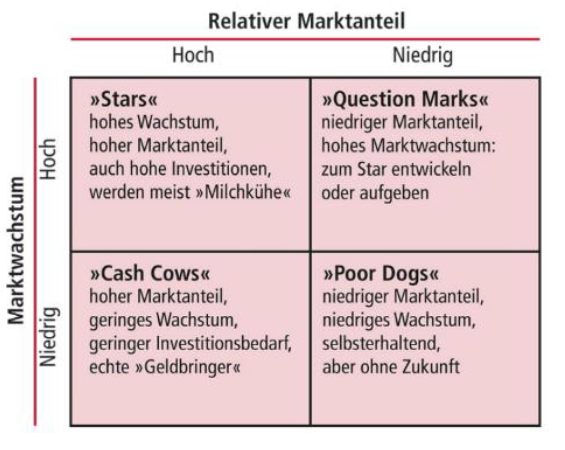
\includegraphics[width=\textwidth,height=0.7\textheight,keepaspectratio]{figures/BCG.png}

    \subsubsection{Produkt-Markt oder Ansoff-Matrix}
    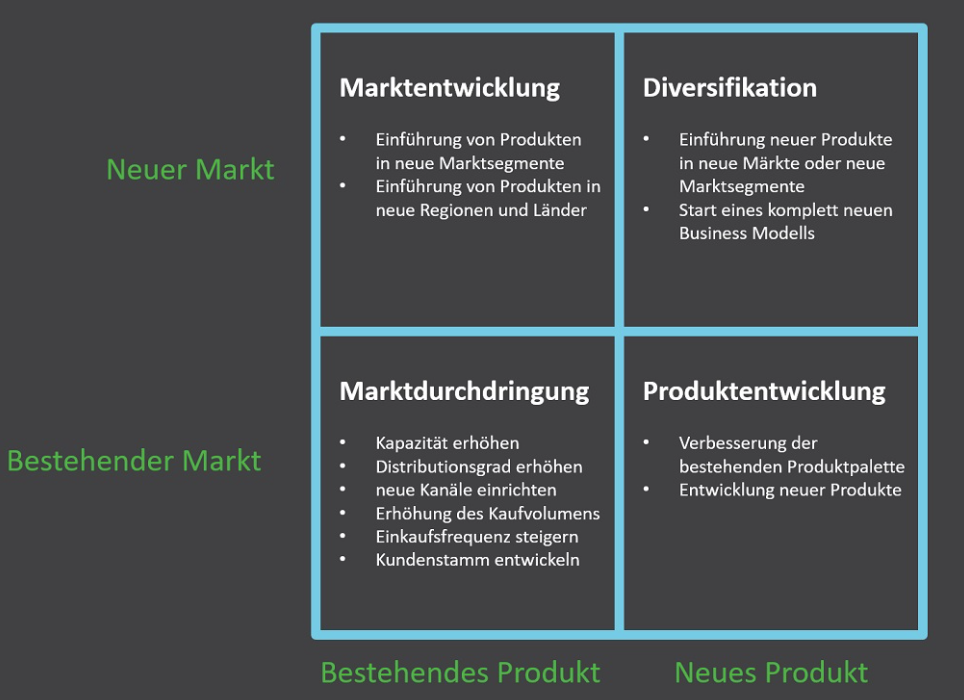
\includegraphics[width=\textwidth,height=0.7\textheight,keepaspectratio]{figures/Ansoff.png}
    

    \section{SWOT Analyse}
    \begin{itemize}
        \item Unternehmensanalyse (intern,mikro)
        \begin{itemize}
            \item Stärken (Gutes Arbeitsumfeld, erfolgreiche Zielgruppe identifizierung)
            \item Schwächen (Kleines Marktpotential, nicht nachhaltig wegen importe)
        \end{itemize}
        \item Umweltanalyse (extern,makro)
        \begin{itemize}
            \item Opportunities (Trend Gesundheit)
            \item Risiken (Konkurrenten Evian usw., Nachhaltigkeit Politik, )
        \end{itemize}
    \end{itemize}

    \subsection{Strategien}
    \begin{itemize}
        \item Matching (Stärken/ maximieren)
        \item Transformation (Schwächen/risiko minimieren)
        \item Neutralität ()
    \end{itemize}
    

\end{document}
